\providecommand{\main}{../..}%define path to bib for subfiles
\documentclass[../../main.tex]{subfiles}
\begin{document}
\onlyinsubfile{\setcounter{chapter}{10}}
\notinsubfile{}
\chapter{styleguide}
\onlyinsubfile{
\marginpar{\vspace{0cm}
\textcolor{red}{ hoofdstuk is los gecompileerd, hstk nummer is 1}}
}
\notinsubfile{
\marginpar{\vspace{0cm}
\textcolor{red}{main.tex gecompileerd, nummering zou moeten kloppen}}
}

juni 2023
Vele typos weggegewerkt (Lianne)
par 2.5 was veel te groot bell test nieuwe paragraph. deze paragraph bevatte een fout. Wiskunde herschreven
 
dec 2022

Inmiddels opgeleverd naar ver NLT.
Overzetten naar github en opschonen van de code.
De dropboxversie met het werk tot nu toe komt in een zip file
(back up)

Alle delen maken gebruik van dezelfde main, preambule en bib files

\begin{verbatim}
directory structuur
kansen met quantum/parts/
kansen met quantum/notes/ %noparts= aantekeningen, geen deel van het boek
kansen met quantum/img
kansen met quantum/bib
\end{verbatim}

\begin{verbatim}
\providecommand{\main}{../..}%define path to bib for subfiles
\documentclass[../../main.tex]{subfiles}
\begin{document}
\onlyinsubfile{\setcounter{chapter}{8}}
\notinsubfile{}
\end{verbatim}

In de notes (nopart) directory staan alle losse aantekeningen. Ze kunnen als stand alone gecompileerd worden met de preambule dankzij bovenstaande codeblock dat bovenin elke file staat.


maart 2022
overgang nieuwe laptop

Met de nieuwe installatie van miktex zijn ook updates uitgevoerd. Net wat meer geheugen nodig. 
PGFplots manual beschrijft dit allemaal (H6). Ik kom er mee weg als in de texmaker configuratie staat:\\
\verb+pdflatex  -synctex=1 -extra-mem-top=7000000 -interaction=nonstopmode %.tex+

Het maximum voor extra-mem-top is trouwens ongeveer 5M6.

bib(la)tex:
texmaker configuration veranderd in:\\  
\verb+"C:/Program Files/MiKTeX/miktex/bin/x64/biber.exe" %+

In de preambule van de tex files staat:\\
\verb+\usepackage[backend=biber,...]{biblatex}+

\href{https://tex.stackexchange.com/questions/154751/biblatex-with-biber-configuring-my-editor-to-avoid-undefined-citations/154788#154788}{check dit op stackexchange}
ik heb ook het usercommando aangepast. Moet wel het volledige pad aangeven (ontbreekt in PATH?

Wellicht handig om de preambule eens op te schonen

Overal wordt lualatex aangeraden en ook external plaatjes

to do: external tikz maken het compileren een stuk sneller.

NB keyboard setting US krijg je deadkeys " followed by space. Zet je keyboard op Canadian english (nog niet gevonden) US doet t ook goed


check alle scource files met notepad++
search all files:
(*.tex in directory quantumtum)

\subsection*{voorbereiden update}
Een update moet een (sub)versienummer verhoging krijgen. Pas die aan in de colofon.
benoem wijzigingen sinds vorige versie.

Geef in main.tex aan welke hoofdstukken en werkbladen opgenomen moeten worden. De directory-structuur incl subrirectories voor afbeeldingen moet je strikt aanhouden.

compileer twee versies docenten en leerlingen. In de preambule moet hiervoor de volgende twee regels worden ingesteld:\\


Voor een docentenversie:\\
\begin{verbatim}
\usepackage{tagging}+\\
%\droptag{teach}%!!!!!!!!!!!!!!!!!!!!!!!!!!!!!!!!!!!!\\
\usetag{teach}%callouts in environment antwoord\
\end{verbatim}

Voor een leerlingeversie
\begin{verbatim}
\usepackage{tagging}
\droptag{teach}%!!!!!!!!!!!!!!!!!!!!!!!!!!!!!!!!!!!!
%\usetag{teach}%callouts in environment antwoord
\end{verbatim}


Compileer main.tex met de quickbuild opties zoals hieronder beschreven (zie texmaker configuratiefiles).


Na het compileren: 
\begin{itemize}[nosep]
\item check op voorkomen van unresolved references ??
\item check bladspiegel pagina voor pagina in beide versies
\item Alles naar github met versienummer
\item lijst met aanpassingen op website en naar NLT
\item upload leerlingenversie naar website 
\item stuur alles naar NLT
\end{itemize}


\textbf{texmaker configuratiefile}


Het package 'subfiles. laat stand-alone compileren van de hoofdstukken toe. Dat scheelt tijd. Daarvoor staat in elk hoofdstuk een kleine preambule.
De hoofdtekst main.tex verwijst naar de hoofdstukken. De directorystructuur luistert nauw.

Het package 'tagging' heeft opdracht droptag en usetag
Selecteer voor het compileren droptech/usetag teach en 
Tekst die met tag 'eruit' is gemekrt kan wel definitief gewist worden.

Ik heb het idee dat main.tex geopend moet zijn om een subfile apart te compileren. Soms doet ie t niet.

Gebruik Quickbuild eerste optie ingesteld (PdfLaTeX + view PDF) om subfiles te compileren.

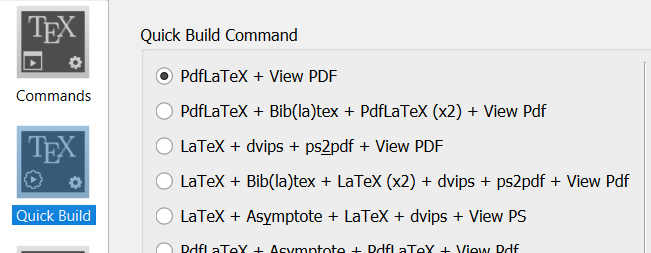
\includegraphics[width=\textwidth]{./img/quickbuild1.PNG}

Gebruik Quickbuild tweede optie (PdfLaTeX +bib(la)tex+PdfLaTex(x)+ View PDF) als alle refereties in orde moeten zijn (hfref alleen verlangt al twee keer compileren). 

compileer main check welke hoofstukken, welke tags


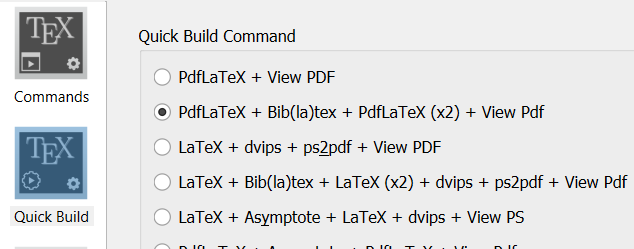
\includegraphics[width=\textwidth]{./img/quickbuild2.PNG}


There may be sections and subsections that have a label but are not referred to. With figs and tables this should not be the case

Unresolved references are errors. Check compiled document on occurrences of \textbf{??}

\textbf{texmaker.ini file}
kopie in directory KmQ (texmaker231010.ini)

\textbf{Enkele compileerfouten}

\verb+! I can't write on file `main.pdf'.+
pdf is nog open -> sluit pdf

\textbf{taal}

verticaal, verticale

Bell-toestand (streepje ertussen)
elektron niet electron

quantumcomputer (niet quantum computer)

twee-toestand systeem twee-toestandsysteem  twee-toestandensysteem, tweetoestandssysteem (tja)

toestandvector (toch maar zonder verbindings -s)

toestandruimte

toestanddiagram

bases niet basen of basissen

het bit= paard

de bit=informatieeenheid  \textbf{toch andersom gedaan. Behalve Van Dale zegt de hele wereld het bit}

de qubit = analoog aan bit (maar iedereen zegt het bit)

eenheidspoort I niet E

quantum (niet kwantum)

dimensionaal niet demensioneel

richtingsco\"effici\"ent 

co\"ordina*
%’ π

zo’n -> zo'n

Tussen de \%'s staat zo'n teken
%%
!Package inputenc Error: Unicode character (U+F020)
(inputenc) not set up for use with LaTeX.
See the inputenc package documentation for explanation.
Type H <return> for immediate help.
...

Hoe zoek je naar chars die buiten de ascii set liggen bijv griekse pi (staat in commentaar
%π
\url{https://design215.com/toolbox/ascii-utf8.php}

met notepad++ kun je zoeken/vervangen in files (*.tex) in een subdir

een regex search "\verb~[^\x00-\x7F]+~" vindt alles buiten de regulaire ascii set

[space]\cite vervangen met [tilde]\cite
\textbf{ascii
}
dingen die vervangen moeten worden
\verb+“” é ë \"e ö \"o ï \"i \'e tab ` ‘ ’ + maar niet in \`e

ë=c3 ab

\verb+’ = e2 80 99+ is een 3-byte character (\url{https://design215.com/toolbox/utf8-3byte-characters.php})


\verb+– = e2 80 93+ 

\verb+… = e2 80 a6+ 

 zo’n
 
 
coëfficiënt gaat goed maar liever \"e gebruiken.

beïnvloeden

 én 
 
 één gaat ook goed, liever  \'e\'en

quotes gewoon " (naast de enter toets met shift)


kansamplitudo’s
Deze gaat mis scheef accent: kansamplitudo's %kansamplitudo’s


package microtype: nog niet gedaan

Koma fonts lukt me niet



\textbf{opmaak}


marginpar

\verb+\marginpar{\vspace{-2cm}\footnotesize{tekst hier }}+

\marginpar{\vspace{-2cm}\footnotesize{%
Richard Feynman:
"And then there's the identity,~\port{I}, which we always have to put in there to complete our mathematics -- it doesn't do a damn thing!"
\cite*[p.476]{feynman1982simulating}
}}

citaten

buitenlands italic


fontsizes
{\tiny tiny}
{\scriptsize scriptsize}
{\footnotesize F-footnotesize.png}
{\small F-small}
{\normalsize F-normalsize.png}
{\large F-large}
{\Large F-large2}
{\LARGE F-large3}
{\huge F-huge}
{\Huge F-huge2}


footnotesize in marginnote.



Augmented learning jaja \hrefqr{www.quantumrules.nl}{quantumrules}

\textbf{environments}

\verb+opdracht+

\verb+experiment+ is gebaseerd op opdracht. 

\verb+antwoord+

\textbf{tags}

\verb+eruit+

\verb+teach+ wordt alleen meegecompileerd  in docentenhandleiding.

tekst 

\textbf{macros's}

\verb+\port{}+

\verb+\nogdoen{}+

\verb+\whereami+ prints odd or even

Hoe gaan 
\verb+\href{}+
en 
\verb+\hrefqr{}+
om met \% tekens in de url?

Het werkt als ik \verb+%+ vervang met \verb+\%+

\textbf{paginaopmaak}

\verb+\notepadlines[5]+ is een macro met een optionele parameter.

voorbeelden van casts
\begin{table}[h]
\begin{tabular}{lllll}
ensuremath:    &\verb+ \ensuremath{1}+& \ensuremath{1}& \ensuremath{a} & \ensuremath{M}  \\
ensuremathvec: &\verb+ \ensuremath{\vec{\mathfrak{1}}}+& \ensuremath{\vec{\mathfrak{1}}}& \ensuremath{\vec{\mathfrak{a}}}&   \ensuremath{\vec{\mathfrak{M}}}\\
ensuremathvec: &\verb+\ensuremath{\vec{1}}+&\ensuremath{\vec{1}}& \ensuremath{\vec{a}}& \ensuremath{\vec{M}}\\
mathvec: &\verb+$\vec{1}$+&$\vec{1}$& $\vec{a}$& $\vec{M}$\\
math bold: &\verb+ \ensuremath{\mathbf{1}}+& \ensuremath{\mathbf{1}}& \ensuremath{\mathbf{a}}& \ensuremath{\mathbf{M}}\\
mathrm{math} bold:&\verb+ $\ensuremath{\mathbf{1}}$+ & $\ensuremath{\mathbf{1}}$ & $\ensuremath{\mathbf{a}}$& $\ensuremath{\mathbf{M}}$\\
bold:&\verb+\textbf{1}+& \textbf{1}& \textbf{a}& \textbf{M}\\
%ensuremath: &\\verb+\ensuremath{\mathscr{1}}&  \ensuremath{\mathscr{a}}&\ensuremath{\mathbb{M}}\\
tensor: &\verb+\textsf{\bfseries{\vect{}V}}+&&&\textsf{\bfseries{\vect{}V}}\\
vect &\verb+ \vect{V}+& \vect{V}& & \\
matr &\verb+ \matr{M}+& \matr{M}& &
\end{tabular}
\end{table}

Enkele definities in main:

\verb+\newcommand*{\vect}[1]{\ensuremath{\vec{#1}}}+

\verb+\newcommand*{\matr}[1]{\ensuremath{#1}}+

\verb+\newcommand*{\port}[1]{\textbf{#1}}+

Een vector schrijf je \vect{v} zo, en een matrix \matr{M} zo en een poort \port{Z} zo.

\textbf{lists:}

Gebruik package \textbf{enumitem}
dan heb je goed contrle over vert spacing.


\textbf{opdrachten}
Antwoord direct boven de opracht niks ertussen, optie om hoogte te verschuiven bv [-1cm]

To do: orphan/widow protectie

\begin{antwoord}[-1cm]
oplossing:
\begin{enumerate}
 \item $M\mqty(1&2\\2&1)$
 \item $\mqty(2\\1)$
\end{enumerate}
\end{antwoord}
\begin{opdracht}
$M\mqty(1\\0)=\mqty(1\\2)$ en $M\mqty(0\\1)=\mqty(2\\1)$
\begin{enumerate}
\item Hoe ziet de matrix er uit?
\item Bereken met de matrix $M\mqty(0\\1)$
\end{enumerate}
\end{opdracht}

\begin{antwoord}[-10cm]
\begin{enumerate}[start=9, wide, labelwidth=!, labelindent=0pt]
\item voor een veel tekst weinig indent
\end{enumerate}
\end{antwoord}

In de werkbladen geen opdrachten. Een werkblad is een opdracht. Daar alleen een genummerde lijst.

In h3 zijn de poorten met subfig aangegeven. Vervangen met minipage?

marginpar kan je niet gebruiken in de mdframded omgevingen (opdracht, experiment, kader). Mdframed is een float. 
marginpar is  een minipage, ook een float. Je mag geen float in een float zetten.

=>gebruik dan marginnote

\marginnote{{\vskip1cm\raggedright
uitlijning marginpar? afhankelijk van de O/E pagina
nieuwe notitie notie ntnot notnot 
\newline nieuwe notitie notie ntnot notnot
nieuwe notitie nieuw}}

kleuren:
zie par 3.1
standaardbasis rood
diagonaal donkergroen 
vectoren blauw

tekst of legenda naast figuur: moet dat met een float?
\begin{flushleft}
%\leavevmode
\begin{minipage}{.35\textwidth}

\begin{tikzpicture}%
\def\ojfrangle{0}
\def\ojobangle{45}
\def\ojscale{.45}
\begin{scope}[scale=\ojscale, rotate=\ojfrangle]
  \draw[thin,red!20] (-5,-5) grid (5,5);
\end{scope}
\end{tikzpicture}
\end{minipage}%
\hfill
\begin{minipage}{.45\textwidth}
\[\begin{aligned}
\ket{D}&=\tfrac{1}{2}\sqrt{2}\ket{H}+\tfrac{1}{2}\sqrt{2}\ket{V}\\
\ket{A}&=\tfrac{1}{2}\sqrt{2}\ket{H}-\tfrac{1}{2}\sqrt{2}\ket{V}\\ 
\ket{H}&=\tfrac{1}{2}\sqrt{2}\ket{D}+\tfrac{1}{2}\sqrt{2}\ket{A}\\
\ket{V}&=\tfrac{1}{2}\sqrt{2}\ket{D}-\tfrac{1}{2}\sqrt{2}\ket{A}\\
\end{aligned}\]%subtiel veel minder whitespace
\captionof{figure}{In de standaardbasis (rood) wordt de zwarte vector met gelijke kans als $\ket{H}$ of $\ket{V}$ waargenomen. In de diagonale basis wordt de vector met zekerheid als $\ket{D}$ waargenomen.}\label{fig:twobases}
\end{minipage}
%\caption{E\'en vector in standaardbasis (rood) en diagonale basis.}\label{fig:hvad}
%\end{figure}
\end{flushleft}

gebruik \textbf{aligned} \verb+aligned+ in H3 een vb met \verb+[-2\baselineskip]+ baselineskip (uitgecommentarieerd)



gebruik \verb+\left(+ en \verb+\right)+ om haakjes in ingewikkelde vergelijkingen te schalen.

uiteindelijke opmaak


whitespace bij formule blokjes bij gebruik \verb+\begin{align}...+

\begin{align}
\ket{D}&=\tfrac{1}{2}\sqrt{2}\ket{H}+\tfrac{1}{2}\sqrt{2}\ket{V}\\
\ket{A}&=\tfrac{1}{2}\sqrt{2}\ket{H}-\tfrac{1}{2}\sqrt{2}\ket{V}\\ 
\ket{H}&=\tfrac{1}{2}\sqrt{2}\ket{D}+\tfrac{1}{2}\sqrt{2}\ket{A}\\
\ket{V}&=\tfrac{1}{2}\sqrt{2}\ket{D}-\tfrac{1}{2}\sqrt{2}\ket{A}
\end{align}%subtiel veel minder whitespace

minder whitespace bij formule blokjes gebruikt \verb+\[\begin{aligned}...+

\[\begin{aligned}
\ket{D}&=\tfrac{1}{2}\sqrt{2}\ket{H}+\tfrac{1}{2}\sqrt{2}\ket{V}\\
\ket{A}&=\tfrac{1}{2}\sqrt{2}\ket{H}-\tfrac{1}{2}\sqrt{2}\ket{V}\\ 
\ket{H}&=\tfrac{1}{2}\sqrt{2}\ket{D}+\tfrac{1}{2}\sqrt{2}\ket{A}\\
\ket{V}&=\tfrac{1}{2}\sqrt{2}\ket{D}-\tfrac{1}{2}\sqrt{2}\ket{A}\\
\end{aligned}\]%subtiel veel minder whitespace

Hier nog wat tekst daarna \verb+\clearpage+

frac of tfrac zoveel mogelijk tfrac


Qircuit
maakt gebruik van xy-pic package
\url{http://home.ustc.edu.cn/~xwchen/Useful%20files/xyguide.pdf}

het commando \verb+\ar@{}+ is heel krachtig gebruik dat om lijntjes te maken.


\clearpage



\begin{flushleft}
\hspace*{-\marginparsep-\marginparwidth}%
\begin{tabular}{|p{\marginparwidth}|p{11cm}|}
\verb+\newpage+& is a low level command on which \verb+\clearpage+ and \verb+\cleardoublepage+ are built upon. It ends the current paragraph (if not issued between paragraphs), fills the current page with white space and starts a new page.\\
\verb+\clearpage+&does something more, as it also flushes the float queues, producing pages of floats if necessary, then starts a new page. \\
\verb+\cleardoublepage+&is the same as \verb+\clearpage+, but it also checks the number of the last ejected page; if the number is odd and twosided typesetting is in force, it fills another blank page so the new page to start on will be again odd-numbered.\\
\verb+\pagebreak+&  is quite different from \verb+\newpage+ and its siblings described above.

If issued inside a paragraph, it will force a page break after the line in which it happens to fall when the paragraph is eventually typeset. It also issues no white space filling command, so the last line on the page will be at the bottom margin when \verb+\flushbottom+ is in force (for instance with \textit{book} or generally with \textit{twosided} documents).

If issued between paragraphs, it will force a page break without filling.

This command is useful in the last stage of document production: one can force a page break at a convenient spot for improving the typesetting of the next page. Clearly, the text should be in definitive form for this to be effective.

Note that \verb+\pagebreak+ has an optional argument, which can be a number among 0, 1, 2, 3, 4. Issuing \verb+\pagebreak[4]+ is the same as \pagebreak, \pagebreak[0] just marks a point where a page break is possible (after the line it falls in). The other numbers mark a greater “desirability” of a page break.
\end{tabular}
\end{flushleft}

opvullen met cartoons

Een lege (even) pagina forceren met 

\verb+\newpage+\\
\verb+%\thispagestyle{empty}+\\
\verb+\mbox{}+

\newpage
\mbox{}


Gebruik een lege \verb+\mbox{}+ want als je \verb+\thispagestyle{empty}+ gebruikt is alles leeg geloof ik

NB Dit lost nog niet op datd e pagina alleen conditioneel even wordt gesckipped

\clearpage

\marginpar{\vspace{-2cm}
\includegraphics[width=0.95\marginparwidth]{./img/smartphone verplicht.png} licht bestaat uit energiepaketjes: fotonen}
marginpar kan niet genest worden in een mdframed block Dan gebruik je marginnote. 
Let op verschil in vertical shift \verb+\vspace{1cm}+ en \verb+\vskip1cm+. (zonder accoladen).
\marginnote{\vskip1cm
\includegraphics[width=0.95\marginparwidth]{./img/smartphone verplicht.png}  tekst hieronder zonder fig referentie is rechts uitgelijnd}




\begin{center}
\leavevmode
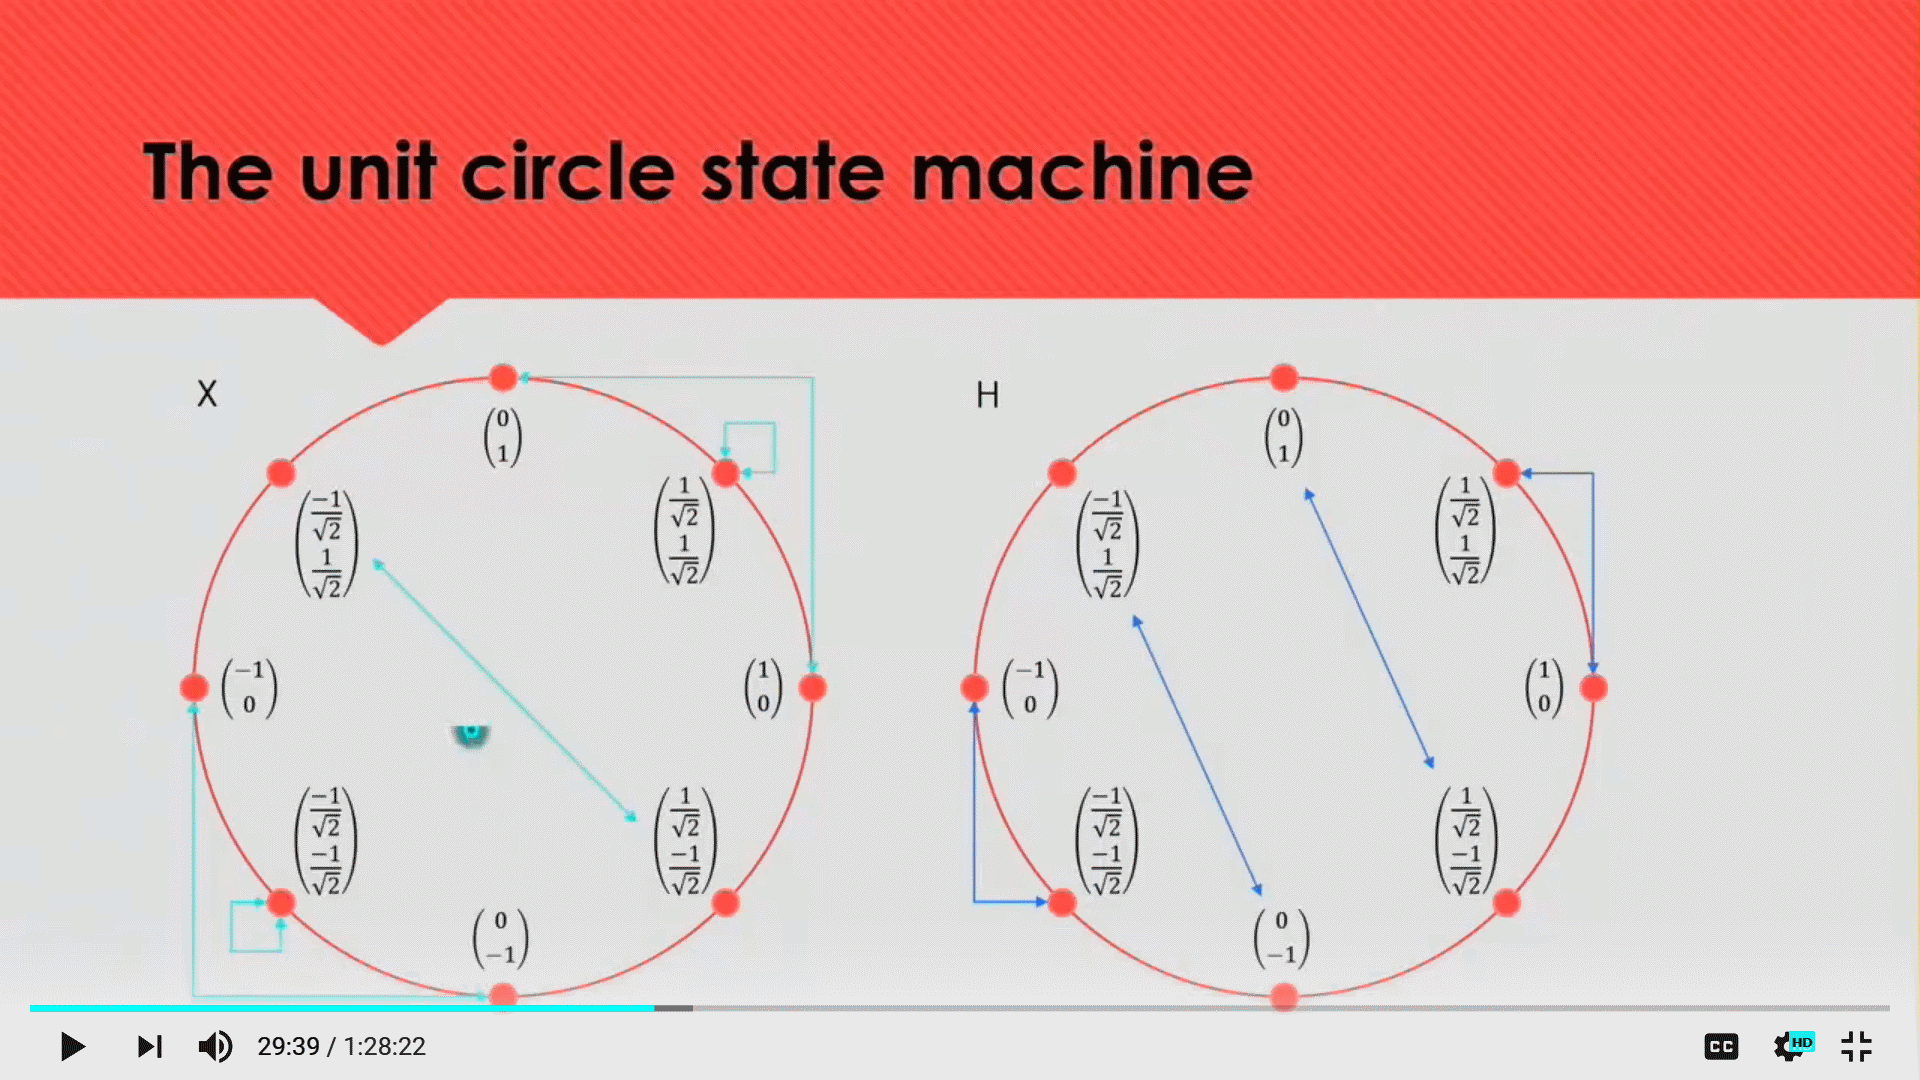
\includegraphics[width=\textwidth+\marginparsep+\marginparwidth, height=1cm]{./img/statemachineXH.png}
\captionof{figure}{Ongepolariseerde fototonen bewegen als transversale golven van rechts naar links. Na het  polarisatiefilter is het licht gepolariseerd. Het filter staat hier onder een hoek van \SI{45}{\degree}. \label{fig:lichtvec}}
\end{center}

tests op even en oneven pagina

fullwitdh figure

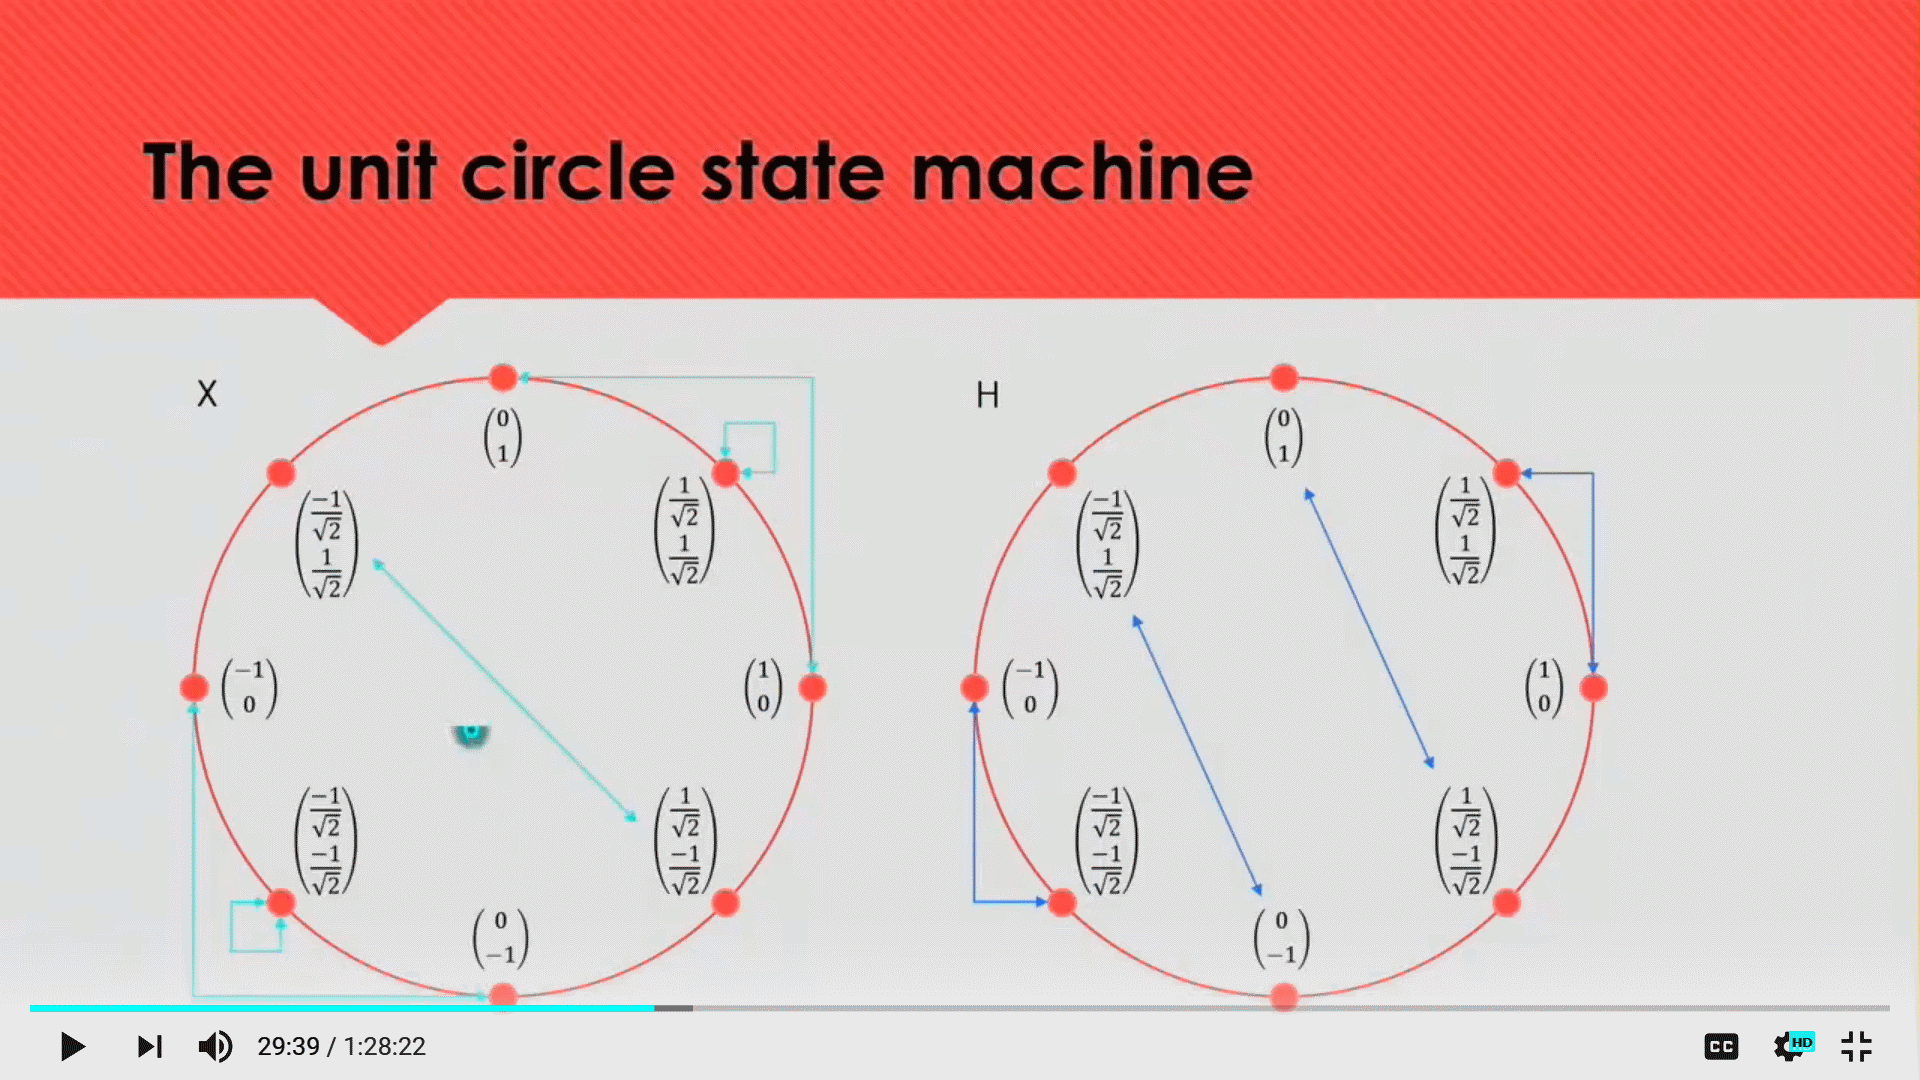
\includegraphics[width=\textwidth, height=1cm]{./img/statemachineXH.png}

\hspace*{0cm}\noindent\makebox{\rule{\linewidth}{0.1pt}}\\
\hspace*{0in}\noindent\makebox{\rule{\textwidth}{0.5pt}}\\
\hspace*{0in}\noindent\makebox{\rule{\textwidth+\marginparsep}{1.pt}}\\
\noindent\makebox{\rule{\textwidth+\marginparsep+\marginparwidth}{1.5pt}}\\
\hspace*{-1.1in}\noindent\makebox{\rule{\paperwidth}{2.0pt}}

notepadlines[5] is een macro met \'e\'en optionele parameter.

\notepadlines[7]


\clearpage
fullwitdh figure even

\checkoddpage\ifoddpage 
  \else 
    \hspace*{-\marginparsep-\marginparwidth}
  \fi%
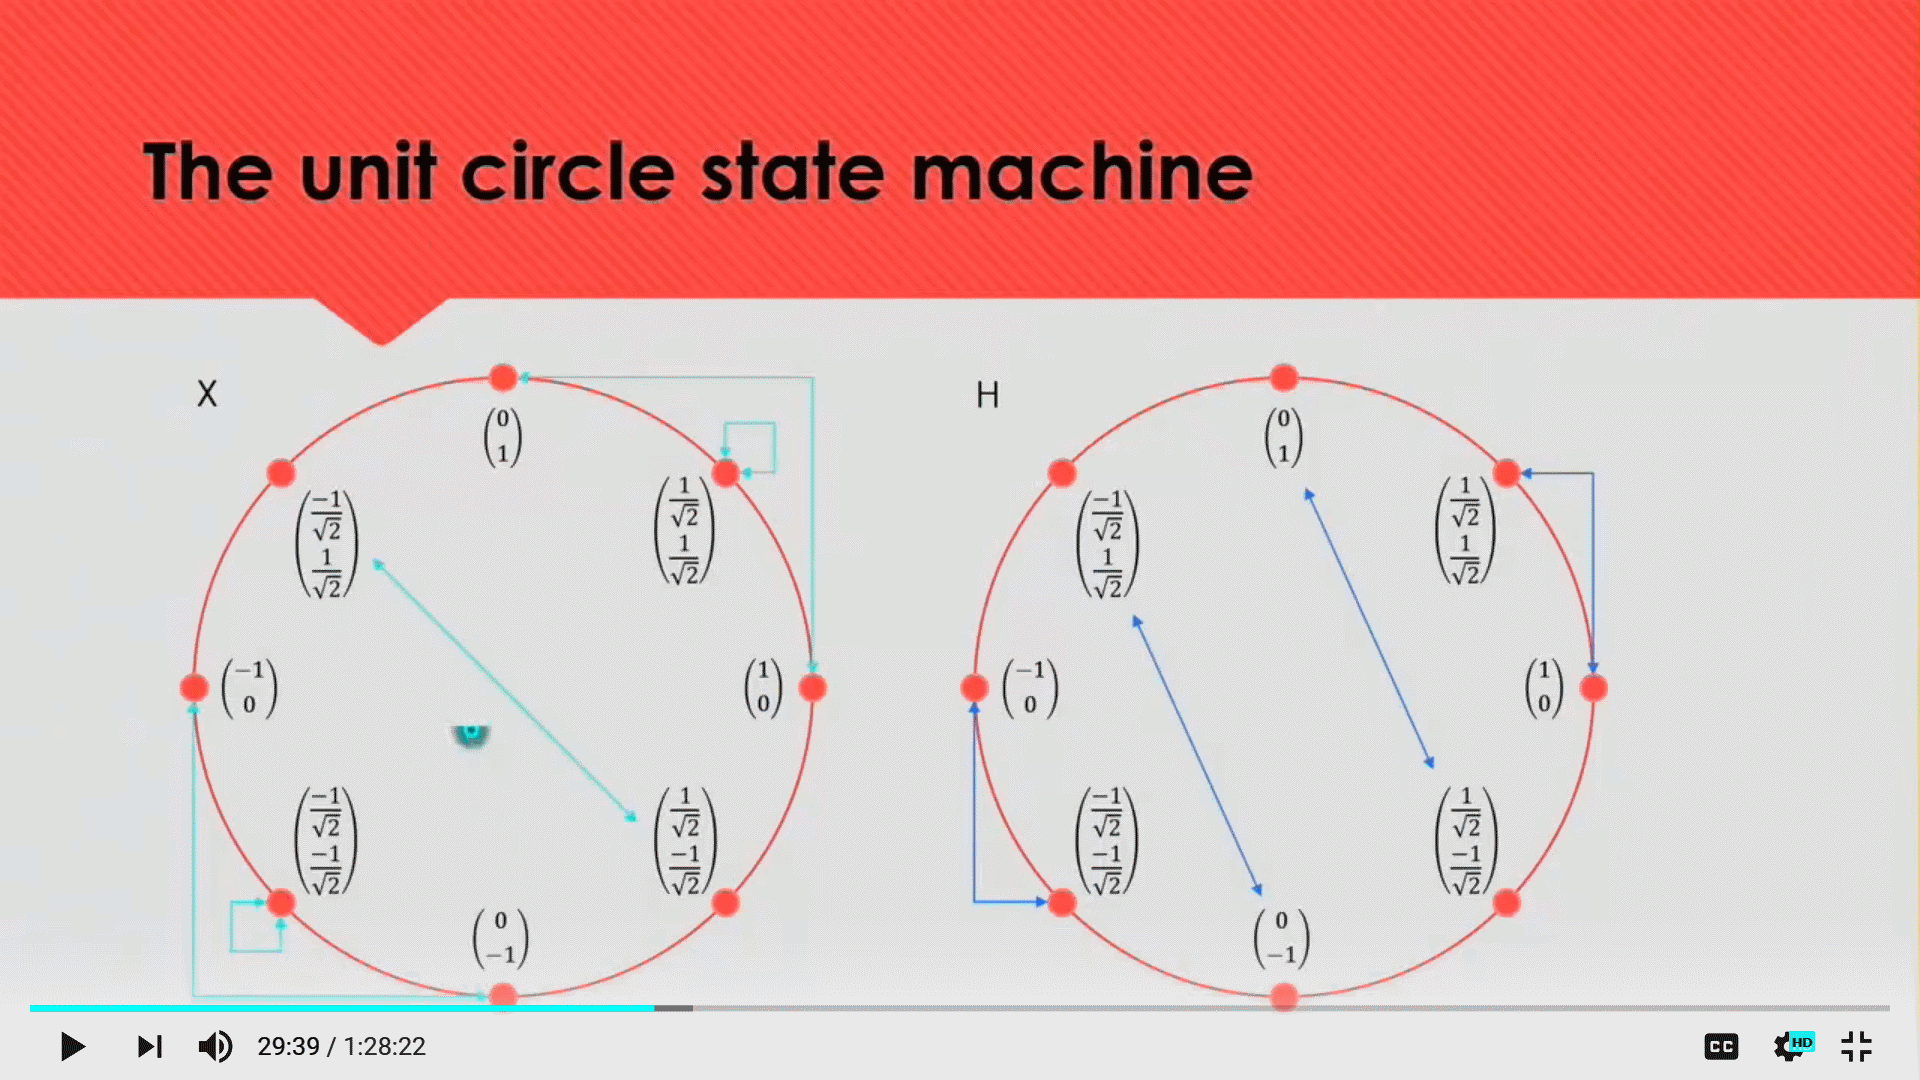
\includegraphics[width=\textwidth+\marginparsep+\marginparwidth, height=1cm]{./img/statemachineXH.png}

\checkoddpage\ifoddpage 
  \else 
    \hspace*{-\marginparsep-\marginparwidth}
  \fi%
\noindent\makebox{\rule{\linewidth}{0.1pt}}\\
\checkoddpage\ifoddpage 
  \else 
    \hspace*{-\marginparsep-\marginparwidth}
  \fi%
\noindent\makebox{\rule{\textwidth}{0.5pt}}\\
\checkoddpage\ifoddpage 
  \else 
    \hspace*{-\marginparsep-\marginparwidth}
  \fi%
\noindent\makebox{\rule{\textwidth+\marginparsep}{1.pt}}\\
\checkoddpage\ifoddpage 
  \else 
    \hspace*{-\marginparsep-\marginparwidth}
  \fi%
\noindent\makebox{\rule{\textwidth+\marginparsep+\marginparwidth}{1.5pt}}\\
\checkoddpage\ifoddpage 
  \else 
    \hspace*{-\marginparsep-\marginparwidth}
  \fi%
\hspace*{-1.1in}%extra binding margin
\noindent\makebox{\rule{\paperwidth}{2.0pt}}

notepadlines

\notepadlines[7]

\checkoddpage\ifoddpage 
    \def\xoff{0in}
  \else 
    \def\xoff{-\marginparsep-\marginparwidth}
  \fi
\noindent dummy text dummy text dummy text dummy text dummy text dummy text dummy text dummy text dummy text dummy text dummy text
\begin{adjustwidth}{\xoff}{0pt}
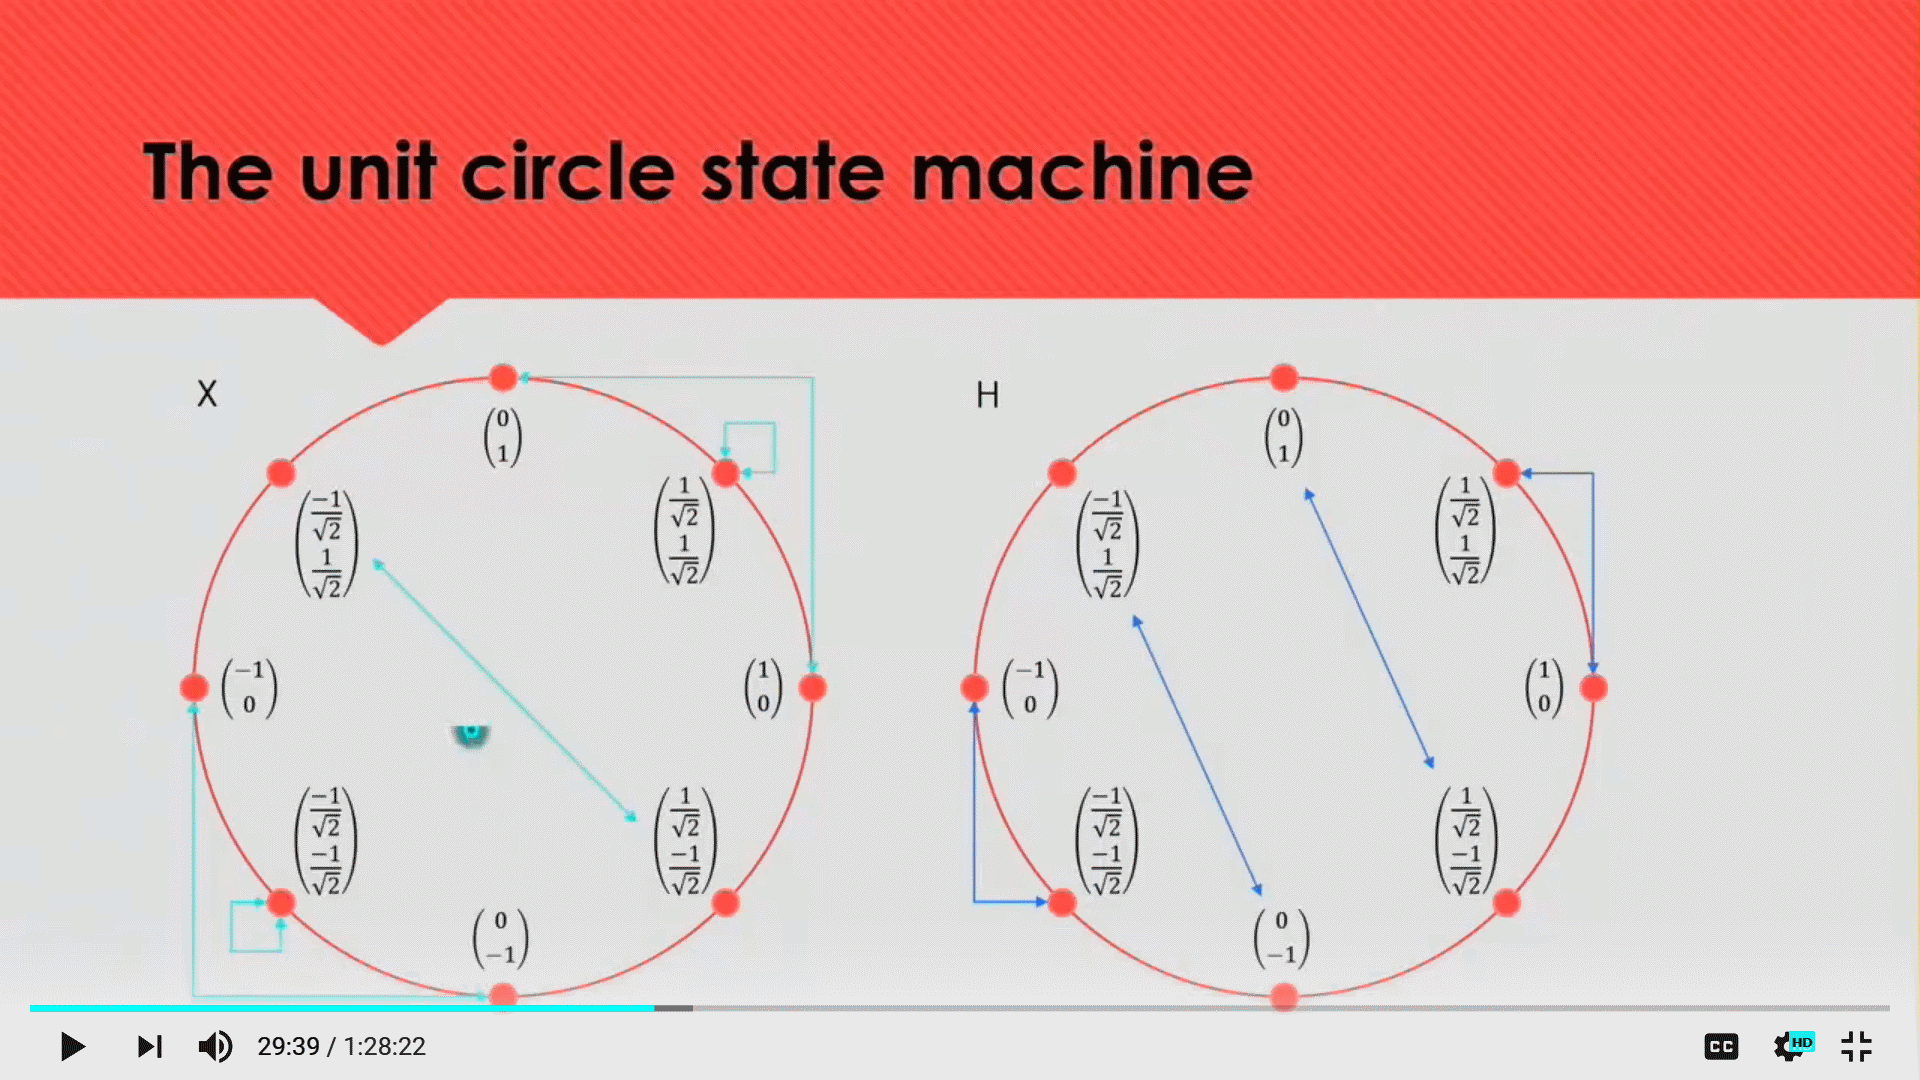
\includegraphics[width=\textwidth+\marginparsep+\marginparwidth, height=1cm]{./img/statemachineXH.png}
\end{adjustwidth}

\clearpage
\noindent adjustwidth adjustwidth adjustwidth adjustwidth adjustwidth adjustwidth adjustwidth adjustwidth adjustwidth
\checkoddpage\ifoddpage 
    \def\xoff{0in}
  \else 
    \def\xoff{-\marginparsep-\marginparwidth}
  \fi
\begin{adjustwidth}{\xoff}{0pt}
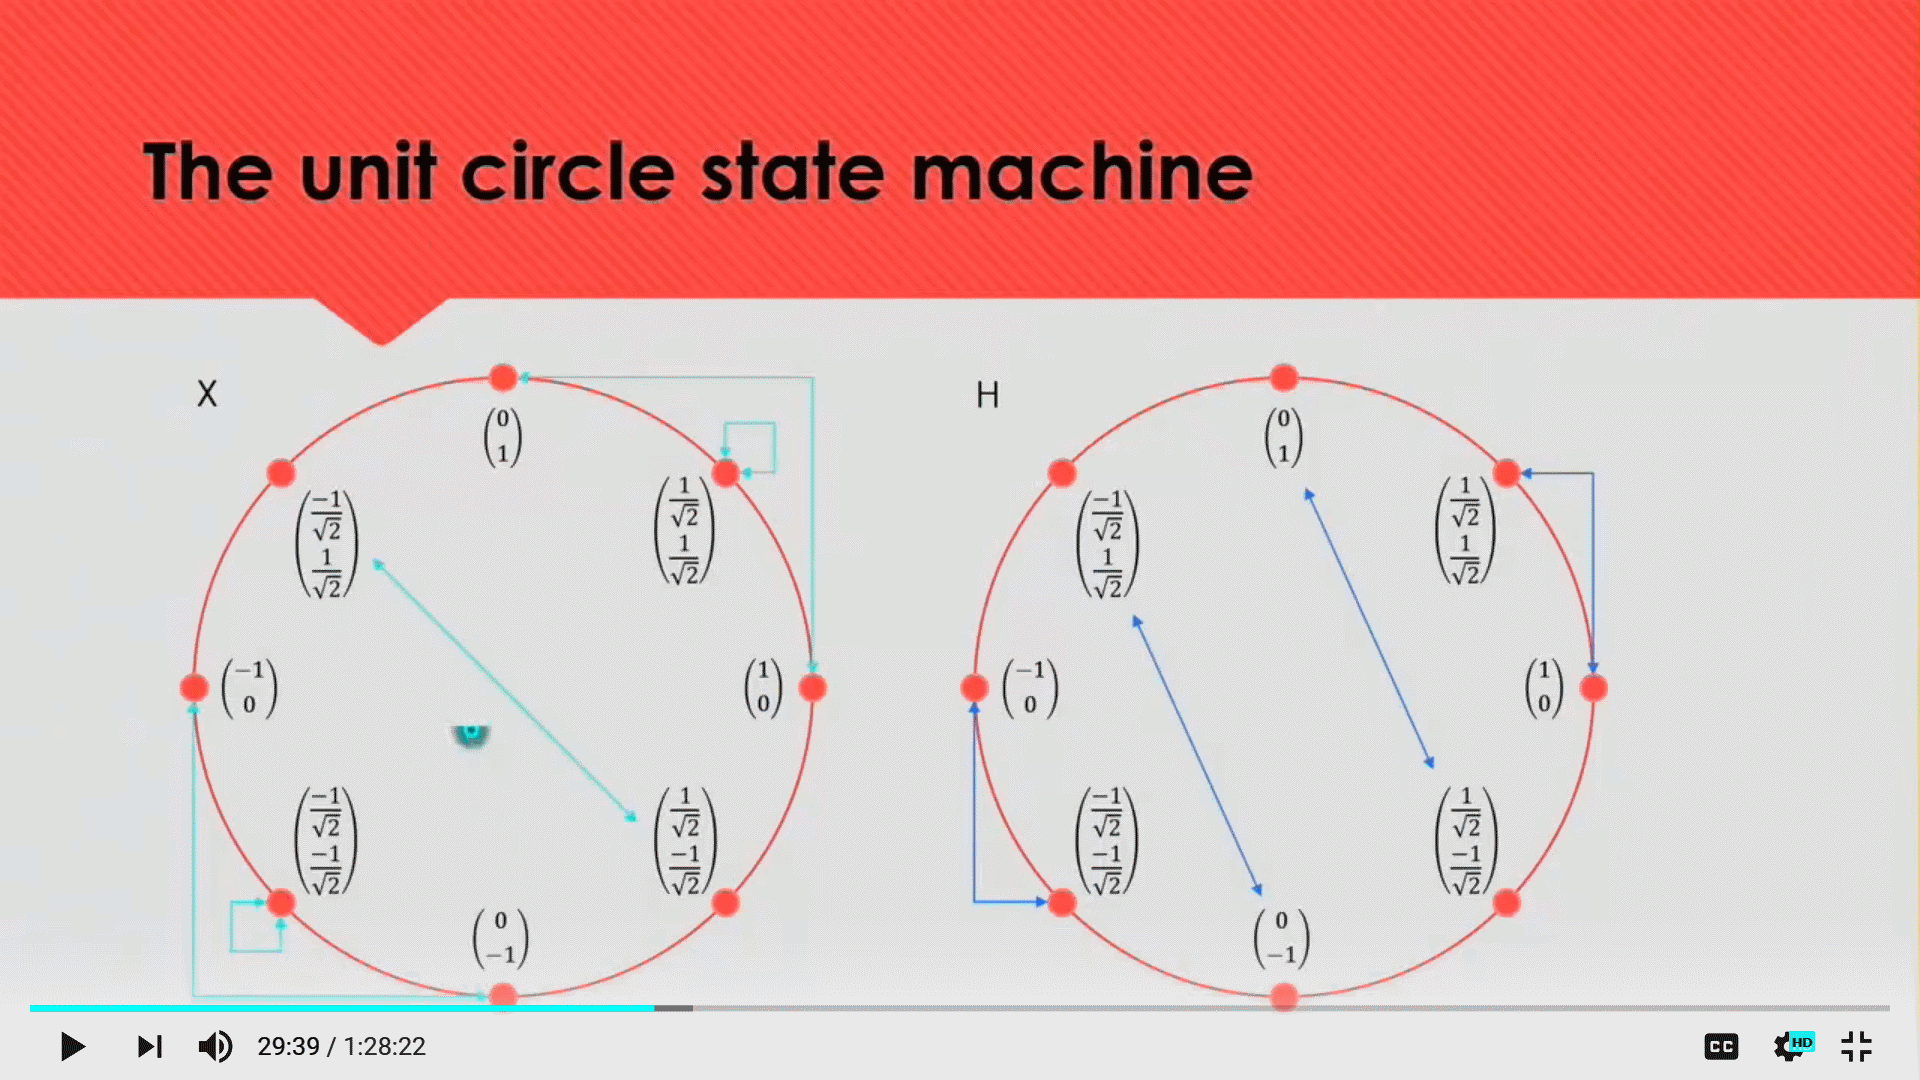
\includegraphics[width=\textwidth+\marginparsep+\marginparwidth, height=1cm]{./img/statemachineXH.png}
\end{adjustwidth}

\clearpage

voorkom afkorten door een \verb+\mbox{}+

list of document parameter settings controlling whitespace

\textbf{pagelayout}\\
\begin{tabular}{p{0.45\textwidth} | p{1.0\textwidth}}
\the\columnsep &\verb:\columnsep: gap between columns\\
\the\topskip &\verb:\topskip: gap above header\\
\the\topskip &\verb:\topskip: between header and text\\
\the\textheight &\verb:\textheight: height of main text\\
\the\textwidth &\verb:\textwidth: width of text\\
\the\oddsidemargin &\verb:\oddsidemargin: odd page left margin\\
\the\evensidemargin &\verb:\evensidemargin : even page left margin\\
\end{tabular}

\textbf{paragraph}\\
\begin{tabular}{p{0.45\textwidth} | p{1.0\textwidth}}
\the\parindent &\verb:\parindent: indentation of paragraphs\\
\the\parskip &\verb:\parskip: gap between paragraphs\\
\end{tabular}

\textbf{floates}\\
\begin{tabular}{p{0.45\textwidth} | p{1.0\textwidth}}
\the\floatsep &\verb:\floatsep: space left between floats.\\
\the\textfloatsep &\verb:\textfloatsep: space between last top float or first bottom float and the text.\\
\the\intextsep &\verb:\intextsep: space left on top and bottom of an in-text float.\\
\the\dbltextfloatsep &\verb+\dbltextfloatsep+ is \verb+\textfloatsep+ for 2 column output.\\
\the\dblfloatsep &\verb+\dblfloatsep+ is \verb+\floatsep+ for 2 column output.\\
\the\abovecaptionskip &\verb:\abovecaptionskip: space above caption\\
\the\belowcaptionskip &\verb:\belowcaptionskip: space below caption\\
\end{tabular}


\textbf{math}\\
\begin{tabular}{p{0.45\textwidth} | p{1.0\textwidth}}
\the\abovedisplayskip & \verb:\abovedisplayskip: space before maths\\
\the\belowdisplayskip & \verb:\belowdisplayskip: space after maths\\
\the\arraycolsep & \verb:\arraycolsep: gap between columns of an array
\end{tabular}


\textbf{Lists}\\
\begin{tabular}{p{0.45\textwidth} | p{1.0\textwidth}}
\the\topsep &\verb:\topsep: space between first item and preceding paragraph.\\
\the\partopsep &\verb:\partopsep: extra space added to \verb+\topsep+ when environment starts a new paragraph.\\
\the\itemsep &\verb:\itemsep: space between successive items.
\end{tabular}

\textbf{sizes}\\
\begin{tabular}{p{0.45\textwidth} | p{1.0\textwidth}}
\the\hoffset&\verb:\hoffset:\\
\the\oddsidemargin&\verb:\oddsidemargin:\\
\the\textwidth &\verb:\\textwidth: .\\
\the\marginparsep &\verb:\marginparsep: .\\
\the\marginparwidth &\verb:\marginparwidth: .\\
\the\paperwidth&\verb:\paperwidth:\\
\\
\the\linewidth&\verb:\linewidth:

\end{tabular}


\clearpage



Voorbeeld tekst naast figuur

\begin{flushleft}
\begin{minipage}{.45\textwidth}

\includegraphics[width=\textwidth]{./img/smartphone verplicht.png}
\end{minipage}%
\hfill
\begin{minipage}{.5\textwidth}
\captionof{figure}{Een foton in de toestand $\ket{1}$ zal het filter passeren.
Een foton in de toestand $\ket{0}$ wordt tegengehouden.
Het foton in de afbeelding heeft een kans van $\cos^2 \theta$ om te worden doorgelaten.\label{fig:photonvector}}
\end{minipage}
%\caption{E\'en vector in standaardbasis (rood) en diagonale basis.}\label{fig:hvad}
%\end{figure}
\end{flushleft}



geometry package geeft alle maten (can only be used in preamble)
staat ook in log file

\the\marginparwidth



Nog altijd ge\"interesseerd in een icon in de marge:

\ref{https://tex.stackexchange.com/questions/444397/inserting-small-icon-or-figure-in-the-margin-left-to-some-desired-title-in-mdfra}

figuur en legenda  naast elkaar. Fbox toegevoegd ter illustratie
minipages tellen op tot maximaal \verb+.95\textwidth+.
\verb+\hfill+ zorgt ervoor dat de fig en legenda naast elkaar staan. Pas op, geen spaties of hardreturn tussen de minipages
.
\begin{flushleft}
%\leavevmode
\fbox{\begin{minipage}{.50\textwidth}
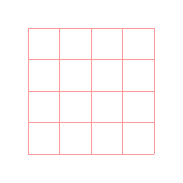
\begin{tikzpicture}
\begin{scope}[scale=.4, rotate=0]
\draw[thin,red!40] (-2,-2) grid (2,2);
\end{scope}
\end{tikzpicture}
\end{minipage}}%
\hfill%hier geen extra linefeeds!!!
\fbox{\begin{minipage}{.45\textwidth}
\captionof{figure}{text hier}\label{fig:dummylabel1}
\end{minipage}}
\fbox{\begin{minipage}{.35\textwidth}
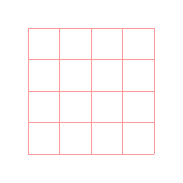
\begin{tikzpicture}
\begin{scope}[scale=.4, rotate=0]
\draw[thin,red!40] (-2,-2) grid (2,2);
\end{scope}
\end{tikzpicture}
%\captionof{figure}{Eenheidscirkel. met eenheidsvecotoren $\ket{0}$ en $\ket{1}$. \label{fig:unitc}}
\end{minipage}}%
\hfill%hier geen extra linefeeds!!!
\begin{minipage}{.45\textwidth}
\captionof{figure}{text hier}\label{fig:dummylabel2}
\end{minipage}
%\caption{E\'en vector in standaardbasis (rood) en diagonale basis.}\label{fig:hvad}
%\end{figure}
\end{flushleft}

Blokje van vier figuren met legenda. Fbox toegevoegd ter illustratie
Begin met een float environment bv flushleft, flushright, center

\begin{flushleft}
\fbox{\begin{minipage}{.50\textwidth}
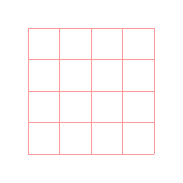
\begin{tikzpicture}
\begin{scope}[scale=.4, rotate=0]
\draw[thin,red!40] (-2,-2) grid (2,2);
\end{scope}
\end{tikzpicture}
\end{minipage}}%
\hfill%hier geen extra linefeeds!!!
\hbox{\begin{minipage}{.45\textwidth}
\captionof{figure}{vervang fbox door hbox of laat fbox weg}\label{fig:dummylabel3}
\end{minipage}}
\fbox{\begin{minipage}{\textwidth}

\begin{tikzpicture}[scale=.1]
\draw[thin,red!40] (-2,-2) grid (2,2);
\end{tikzpicture}
\end{minipage}}%
\hfill%hier geen extra linefeeds!!!
\fbox{\begin{minipage}{.3\textwidth}
\small{ niet genummerd gebruik small}\label{fig:dummylabel4}
\end{minipage}}
\fbox{\begin{minipage}{\textwidth}
\captionof{figure}{text onder, he textwidth is te breed}\label{fig:dummylabel5}
\end{minipage}}
\end{flushleft}

\begin{center}
\mbox{\begin{minipage}{\textwidth}

\begin{tikzpicture}[scale=.1]
\draw[thin,red!40] (-2,-2) grid (2,2);
\end{tikzpicture}
\end{minipage}}%
\hfill%hier geen extra linefeeds!!!
\mbox{\begin{minipage}{.3\textwidth}
niet genummerd\label{fig:dummylabel6}
\end{minipage}}

\fbox{\begin{minipage}{.5\textwidth}
\small{gebruik mbox, niet hbox zonder frame}\label{fig:dummylabel7}
\end{minipage}}
\end{center}

Wrapfigure is mischien toch wel een mooi package. Met hoofdletters {RLIO} is het een float, met kleine lettere {rlio} niet. Je kan ook overhang aangeven. in het voorbeeld ook vskip grbruikt. en een tekst zonder figuurnummering.
ectus vestibulum urna fringilla ultrices.  Phasellus eu tellus sit amet 
tortor gravida placerat. Integer sapien est, iaculis in, pretium quis, 
viverra ac, nunc. Praesent eget sem vel leo ultrices bibendum. Aenean 
faucibus.
\verb+[〈nr of narrow lines〉]{〈placement〉}[〈overhang〉] {〈width〉}+
\begin{wrapfigure}%
{o}% overhang kleine letter geen ftoat
[\marginparwidth+\marginparsep]%overhang
{0.45\textwidth}%width
\centering
\vskip0cm

\includegraphics[width=0.35\textwidth]{./img/smartphone verplicht.png}
 \captionof{figure}{ kies r,R l,L, iI oO overhang en een beetje vskip
\label{fig:wrap}}

\end{wrapfigure}
Morbi dolor nulla, malesuada eu, pulvinar at, mollis ac, nulla. Curabitur 
auctor semper nulla. Donec varius orci eget risus. Duis nibh mi, congue eu, 
accumsan eleifend, sagittis quis, diam. Duis eget orci sit amet orci 
dignissim rutrum.



In hoofstuk 1 staat een voorbeeld (figuur met gepolariseerd licht) hoe je de plaatsing van een figuur in de marge kunt uitbreiden.
H3 quantuamprotocollen



\end{document}
